\documentclass[amsmath, amssymb, aip, jmp, reprint]{revtex4-2}
\usepackage{tikz}
\usetikzlibrary{shapes.geometric}
\usetikzlibrary{decorations.markings}

\begin{document}

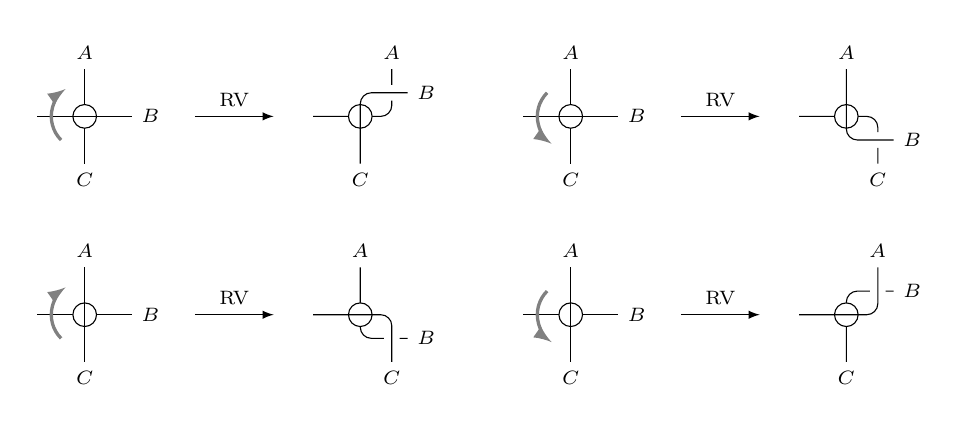
\begin{tikzpicture}[> = latex, font = \scriptsize]
\matrix[column sep = 1 cm, row sep = 0.5 cm]{

	% Original vertex with edges

	\draw (0, -0.6) node [below] {$C$} -- (0, 0.6) node [above] {$A$};
	\draw [fill = white] (0, 0) circle (0.15);
	\draw (-0.6, 0) -- (0.6, 0) node [right] {$B$};

	\draw [->, very thick, gray] (-0.3, -0.3) arc (225 : 125 : {0.3 * sqrt(2)});

	\draw [->] (1.4, 0) -- node [above] {RV} (2.4, 0);

	% New vertex after rotation

	\draw [rounded corners] (2.9, 0) -- (3.9, 0) -- (3.9, 0.2) (3.9, 0.4) -- (3.9, 0.6) node [above] {$A$};
	\draw [fill = white] (3.5, 0) circle (0.15);
	\draw [rounded corners] (3.5, -0.6) node [below] {$C$} -- (3.5, 0.3) -- (4.1, 0.3) node [right] {$B$};

&

	% Original vertex with edges

	\draw (0, -0.6) node [below] {$C$} -- (0, 0.6) node [above] {$A$};
	\draw [fill = white] (0, 0) circle (0.15);
	\draw (-0.6, 0) -- (0.6, 0) node [right] {$B$};

	\draw [->, very thick, gray] (-0.3, 0.3) arc (135 : 235 : {0.3 * sqrt(2)});

	\draw [->] (1.4, 0) -- node [above] {RV} (2.4, 0);

	% New vertex after rotation

	\draw [rounded corners] (2.9, 0) -- (3.9, 0) -- (3.9, -0.2) (3.9, -0.4) -- (3.9, -0.6) node [below] {$C$};
	\draw [fill = white] (3.5, 0) circle (0.15);
	\draw [rounded corners] (3.5, 0.6) node [above] {$A$} -- (3.5, -0.3) -- (4.1, -0.3) node [right] {$B$};

\\

	% Original vertex with edges

	\draw (-0.6, 0) -- (0.6, 0) node [right] {$B$};
	\draw [fill = white] (0, 0) circle (0.15);
	\draw (0, -0.6) node [below] {$C$} -- (0, 0.6) node [above] {$A$};

	\draw [->, very thick, gray] (-0.3, -0.3) arc (225 : 125 : {0.3 * sqrt(2)});

	\draw [->] (1.4, 0) -- node [above] {RV} (2.4, 0);

	% New vertex after rotation

	\draw [rounded corners] (3.5, 0.6) node [above] {$A$} -- (3.5, -0.3) -- (3.8, -0.3) (4, -0.3) -- (4.1, -0.3) node [right] {$B$};
	\draw [fill = white] (3.5, 0) circle (0.15);
	\draw [rounded corners] (2.9, 0) -- (3.9, 0) -- (3.9, -0.6) node [below] {$C$};

&

	% Original vertex with edges

	\draw (-0.6, 0) -- (0.6, 0) node [right] {$B$};
	\draw [fill = white] (0, 0) circle (0.15);
	\draw (0, -0.6) node [below] {$C$} -- (0, 0.6) node [above] {$A$};

	\draw [->, very thick, gray] (-0.3, 0.3) arc (135 : 235 : {0.3 * sqrt(2)});

	\draw [->] (1.4, 0) -- node [above] {RV} (2.4, 0);

	% New vertex after rotation

	\draw [rounded corners] (3.5, -0.6) node [below] {$C$} -- (3.5, 0.3) -- (3.8, 0.3) (4, 0.3) -- (4.1, 0.3) node [right] {$B$};
	\draw [fill = white] (3.5, 0) circle (0.15);
	\draw [rounded corners] (2.9, 0) -- (3.9, 0) -- (3.9, 0.6) node [above] {$A$};

\\
};

\end{tikzpicture}

\end{document}